% Relatório do TP "Analisando Grafos do SNAP" -- Grafo G99 (CollegeMsg)
% Compilar no Overleaf com o template WebMedia (webmedia.cls). Os números vêm de macros.tex
% (gerado por scripts/run_all.py) e as tabelas de tabelas/*.tex (gerado por scripts/gerar_tabelas_tex.py).
\documentclass[sigconf]{webmedia}

\usepackage[brazilian]{babel}
\usepackage{booktabs}
% gerado automaticamente por scripts/run_all.py
\newcommand{\nNos}{1.899}
\newcommand{\nMensagens}{59.835}
\newcommand{\nArestasDir}{20.296}
\newcommand{\nArestasND}{13.838}
\newcommand{\nDias}{193,7}
\newcommand{\grauMin}{1}
\newcommand{\grauMax}{255}
\newcommand{\grauMedio}{14,57}
\newcommand{\grauMediana}{5}
\newcommand{\densidade}{0,00768}
\newcommand{\reciprocidade}{63,6\%}
\newcommand{\nComponentes}{4}
\newcommand{\tamMaiorComp}{1.893}
\newcommand{\diametro}{8}
\newcommand{\raio}{4}
\newcommand{\caminhoMedio}{3,055}
\newcommand{\clustMedio}{0,109}
\newcommand{\transitividade}{0,057}
\newcommand{\nTriangulos}{14.319}
\newcommand{\coreMax}{20}
\newcommand{\assortatividade}{-0,188}
\newcommand{\sigmaER}{14,5}
\newcommand{\sigmaGrau}{1,23}
\newcommand{\razaoCER}{14,4}
\newcommand{\razaoLER}{0,991}
\newcommand{\razaoCGrau}{1,24}
\newcommand{\razaoLGrau}{1,006}
\newcommand{\gammaPL}{2,83}
\newcommand{\kminPL}{35}
\newcommand{\nCaudaPL}{214}
\newcommand{\pvalorPL}{0,02}
\newcommand{\gammaOLS}{1,33}
\newcommand{\RLognormal}{-3,9}
\newcommand{\pLognormal}{0,07}
\newcommand{\RExponencial}{2,0}
\newcommand{\pExponencial}{0,71}
\newcommand{\nRemovidos}{95}
\newcommand{\AAleatorio}{0,939}
\newcommand{\ARelAleatorio}{0,989}
\newcommand{\BAleatorio}{20,8}
\newcommand{\CAleatorio}{3,064}
\newcommand{\DAleatorio}{1,1\%}
\newcommand{\AAtaqueGrau}{0,793}
\newcommand{\BAtaqueGrau}{289}
\newcommand{\CAtaqueGrau}{3,795}
\newcommand{\DAtaqueGrau}{15,6\%}
\newcommand{\AAtaqueInterm}{0,763}
\newcommand{\BAtaqueInterm}{339}
\newcommand{\CAtaqueInterm}{3,698}
\newcommand{\DAtaqueInterm}{18,1\%}
\newcommand{\AAtaquePR}{0,827}
\newcommand{\BAtaquePR}{228}
\newcommand{\CAtaquePR}{3,618}
\newcommand{\DAtaquePR}{12,3\%}
\newcommand{\nPontes}{395}
\newcommand{\nArticulacoes}{220}
\newcommand{\nSCC}{601}
\newcommand{\maiorSCC}{1294}
\newcommand{\grausImpares}{1062}
\newcommand{\pesoMST}{746,15}
\newcommand{\topCincoMsgs}{47,0\%}
\newcommand{\primeirasOitoSem}{79,7\%}


\setcopyright{none}
\settopmatter{printacmref=false}
\renewcommand\footnotetextcopyrightpermission[1]{}

\begin{document}

\title[Grafo G99 -- CollegeMsg]{Análise do Grafo G99 (CollegeMsg) do SNAP: Estrutura, Algoritmos e Propriedades de Redes Complexas}

% TODO: preencher nome completo e e-mail
\author{Nome Completo da Aluna}
\affiliation{%
  \institution{Universidade Federal da Bahia}
  \city{Salvador}
  \state{BA}
  \country{Brasil}}
\email{email@ufba.br}

\renewcommand{\shortauthors}{Nome Completo da Aluna}

\begin{abstract}
Este trabalho analisa o grafo G99 da coleção SNAP, a rede temporal de mensagens privadas \emph{CollegeMsg}, atribuída pela matrícula 224215941. Após converter a rede temporal em um grafo estático simples, caracterizamos sua estrutura (\nNos{} vértices, \nArestasND{} arestas não dirigidas), implementamos à mão os algoritmos clássicos de busca, caminhos mínimos, componentes e árvore geradora mínima, medindo seus tempos com intervalos de confiança, e investigamos mundo pequeno, lei de potência e robustez a falhas e ataques. A rede tem caminhos curtos (média \caminhoMedio) e agrupamento muito acima do esperado ao acaso, mas essa diferença se reduz a $\approx$\sigmaGrau{} quando se preservam os graus; a lei de potência é rejeitada ($p=\pvalorPL$); e a rede é robusta a falhas aleatórias, porém frágil a ataques a hubs. O código, os dados tratados e os testes estão no repositório público do trabalho.
\end{abstract}

\keywords{teoria dos grafos, redes complexas, mundo pequeno, lei de potência, robustez, SNAP}

\maketitle

%--------------------------------------------------------------------
\section{Introdução}
Este relatório descreve a análise do grafo atribuído ao autor no trabalho prático \emph{Analisando Grafos do SNAP} da disciplina de Teoria dos Grafos. O trabalho tem três partes: (I) caracterização estrutural; (II) implementação e medição de algoritmos clássicos; e (III) investigação de propriedades de redes complexas (mundo pequeno, lei de potência, robustez). Todas as medidas foram calculadas com código próprio, e as bibliotecas prontas (NetworkX~\cite{hagberg2008}) foram usadas apenas para validar os resultados nos testes automatizados.

\subsection*{Determinação do grafo}
A função de atribuição é $f(M) = \big(S(M)\cdot(U(M)+1)\big) \bmod 129$, com $S$ a soma dos dígitos da matrícula e $U$ seus dois últimos dígitos (resultado 0 equivale a 129). Para $M = 224215941$:
\begin{equation}
  S = 2+2+4+2+1+5+9+4+1 = 30, \quad U = 41,
\end{equation}
\begin{equation}
  f(M) = (30\cdot 42) \bmod 129 = 1260 \bmod 129 = 99.
\end{equation}
O grafo é, portanto, o \textbf{G99 = CollegeMsg}, mensagens privadas trocadas em uma rede social de estudantes da Universidade da Califórnia em Irvine~\cite{panzarasa2009,snap}.

\subsection*{Repositório}
Código, dados tratados, testes e instruções de execução estão em: \url{https://github.com/USUARIO/REPOSITORIO} % TODO: trocar pelo link real após o push

\section{Grafo original e tratamento dos dados}
\subsection{Descrição do grafo original}
O arquivo \texttt{CollegeMsg.txt} tem uma linha por mensagem, no formato \texttt{origem destino instante}. São \nMensagens{} mensagens entre \nNos{} usuários ao longo de \nDias{} dias. Trata-se de um grafo temporal dirigido e um multigrafo, pois o mesmo par pode trocar muitas mensagens (Figura~\ref{fig:atividade}).

Os números publicados pelo SNAP divergem entre a tabela-índice e a página do conjunto: as colunas de arestas temporais e estáticas aparecem trocadas na tabela-índice. Contamos diretamente no arquivo e adotamos esses valores: \nMensagens{} arestas temporais e \nArestasDir{} arestas estáticas dirigidas (pares únicos origem$\to$destino).

\begin{figure}[t]
  \centering
  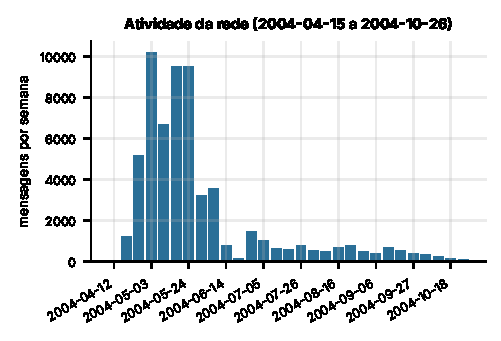
\includegraphics[width=\columnwidth]{figuras/atividade_semanal.pdf}
  \caption{Mensagens por semana. A atividade se concentra no início do período: \primeirasOitoSem{} das mensagens ocorrem nas oito primeiras semanas.}
  \Description{Gráfico de barras com o número de mensagens por semana, decrescente ao longo do tempo.}
  \label{fig:atividade}
\end{figure}

\subsection{Tratamento}
Aplicamos, nesta ordem, os tratamentos da Tabela~\ref{tab:tratamento}: (i) remoção de auto-laços (nenhum encontrado); (ii) colapso do multigrafo em grafo simples, com uma aresta por par; (iii) versão não dirigida, com aresta $\{u,v\}$ se existe $u\to v$ ou $v\to u$; (iv) peso $w=1/m$, em que $m$ é o número de mensagens do par, de modo que pares que conversam mais ficam \emph{mais próximos} (peso positivo, necessário para Dijkstra); (v) restrição à maior componente conexa para as medidas de distância, com \tamMaiorComp{} vértices. Os dois formatos tratados estão versionados em \texttt{data/processed/}.

\begin{table}
  \caption{Etapas do tratamento: tamanho do grafo após cada etapa.}
  \label{tab:tratamento}
  \small
  \begin{tabular}{p{4.2cm}rr}
    \toprule
    Etapa & Vértices & Arestas \\
    \midrule
    Arquivo original (1 linha = 1 mensagem) & 1.899 & 59.835 \\
    Remoção de auto-loops & 1.899 & 59.835 \\
    Grafo estático simples dirigido & 1.899 & 20.296 \\
    Grafo estático simples não dirigido & 1.899 & 13.838 \\
    Maior componente conexa & 1.893 & 13.835 \\
    \bottomrule
  \end{tabular}
\end{table}


\section{Metodologia}
Todos os algoritmos foram implementados em Python puro (\texttt{src/}), e cada um é comparado com o NetworkX nos 28 testes automatizados, inclusive em casos construídos (ciclo negativo, grafo desconexo, grafos eulerianos). A semente aleatória é fixa (42).

\paragraph{Parte I.} Diâmetro, raio e caminho médio são exatos, por BFS a partir de cada vértice da maior componente. Clusterização média, transitividade, triângulos, núcleos $k$, assortatividade e reciprocidade são exatos.

\paragraph{Parte II.} Cada algoritmo é executado 30 vezes (5 para Floyd--Warshall), descartando uma execução de aquecimento e com o coletor de lixo desativado. Reportamos média, desvio-padrão e IC de 95\%, calculado pela distribuição Normal quando $n\ge30$ e pela t-Student quando $n<30$. O crescimento observado é estimado pela inclinação do ajuste log-log do tempo em amostras crescentes de vértices.

\paragraph{Parte III.} \emph{Mundo pequeno:} comparamos $C$ e $L$ com dois nulos, o aleatório $G(n,m)$~\cite{erdos1959} e o de mesmos graus (religações com preservação do grau~\cite{maslov2002}), e usamos o critério $L\approx L_{al}$ e $C\gg C_{al}$ de~\cite{watts1998}, resumido por $\sigma=(C/C_{al})/(L/L_{al})$~\cite{humphries2008}. \emph{Lei de potência:} estimativa por máxima verossimilhança discreta com $k_{\min}$ escolhido por KS, $p$-valor por \emph{bootstrap} e razão de verossimilhanças de Vuong~\cite{vuong1989} contra exponencial e lognormal~\cite{clauset2009}. \emph{Robustez:} removemos $r=\lceil 0{,}05\,n\rceil=\nRemovidos$ vértices, ao acaso (30 repetições) ou segundo um ranking fixo por grau, intermediação (Brandes~\cite{brandes2001}) ou PageRank~\cite{page1999}, e medimos A (fração na maior componente), B (número de componentes), C (caminho médio) e D (fração de isolados)~\cite{albert2000}.

%--------------------------------------------------------------------
\section{Resultados: Parte I}
A rede tem \nNos{} vértices e \nArestasDir{} arestas dirigidas (\nArestasND{} não dirigidas). Os graus vão de \grauMin{} a \grauMax{}, com média \grauMedio{} e mediana \grauMediana{}, e a densidade é de apenas \densidade{} (Tabela~\ref{tab:medidas}). A distribuição é muito assimétrica (Figura~\ref{fig:graus}): poucos usuários concentram muitas conexões. Há \nComponentes{} componentes (tamanhos 1893, 2, 2 e 2); a maior contém quase todos os vértices.

\begin{table}[t]
  \caption{Medidas da Parte I. Distâncias calculadas na maior componente.}
  \label{tab:medidas}
  \small
  \begin{tabular}{lr}
    \toprule
    Medida & Valor \\
    \midrule
    Vértices & \nNos \\
    Arestas (dirigido / não dirigido) & \nArestasDir{} / \nArestasND \\
    Grau mínimo / máximo / médio & \grauMin{} / \grauMax{} / \grauMedio \\
    Densidade & \densidade \\
    Componentes conexas & \nComponentes \\
    Diâmetro / raio & \diametro{} / \raio \\
    Caminho médio & \caminhoMedio \\
    Clusterização média & \clustMedio \\
    Transitividade & \transitividade \\
    Triângulos & \nTriangulos \\
    Núcleo $k$ máximo & \coreMax \\
    Assortatividade de grau & \assortatividade \\
    Reciprocidade & \reciprocidade \\
    \bottomrule
  \end{tabular}
\end{table}

\begin{figure}[t]
  \centering
  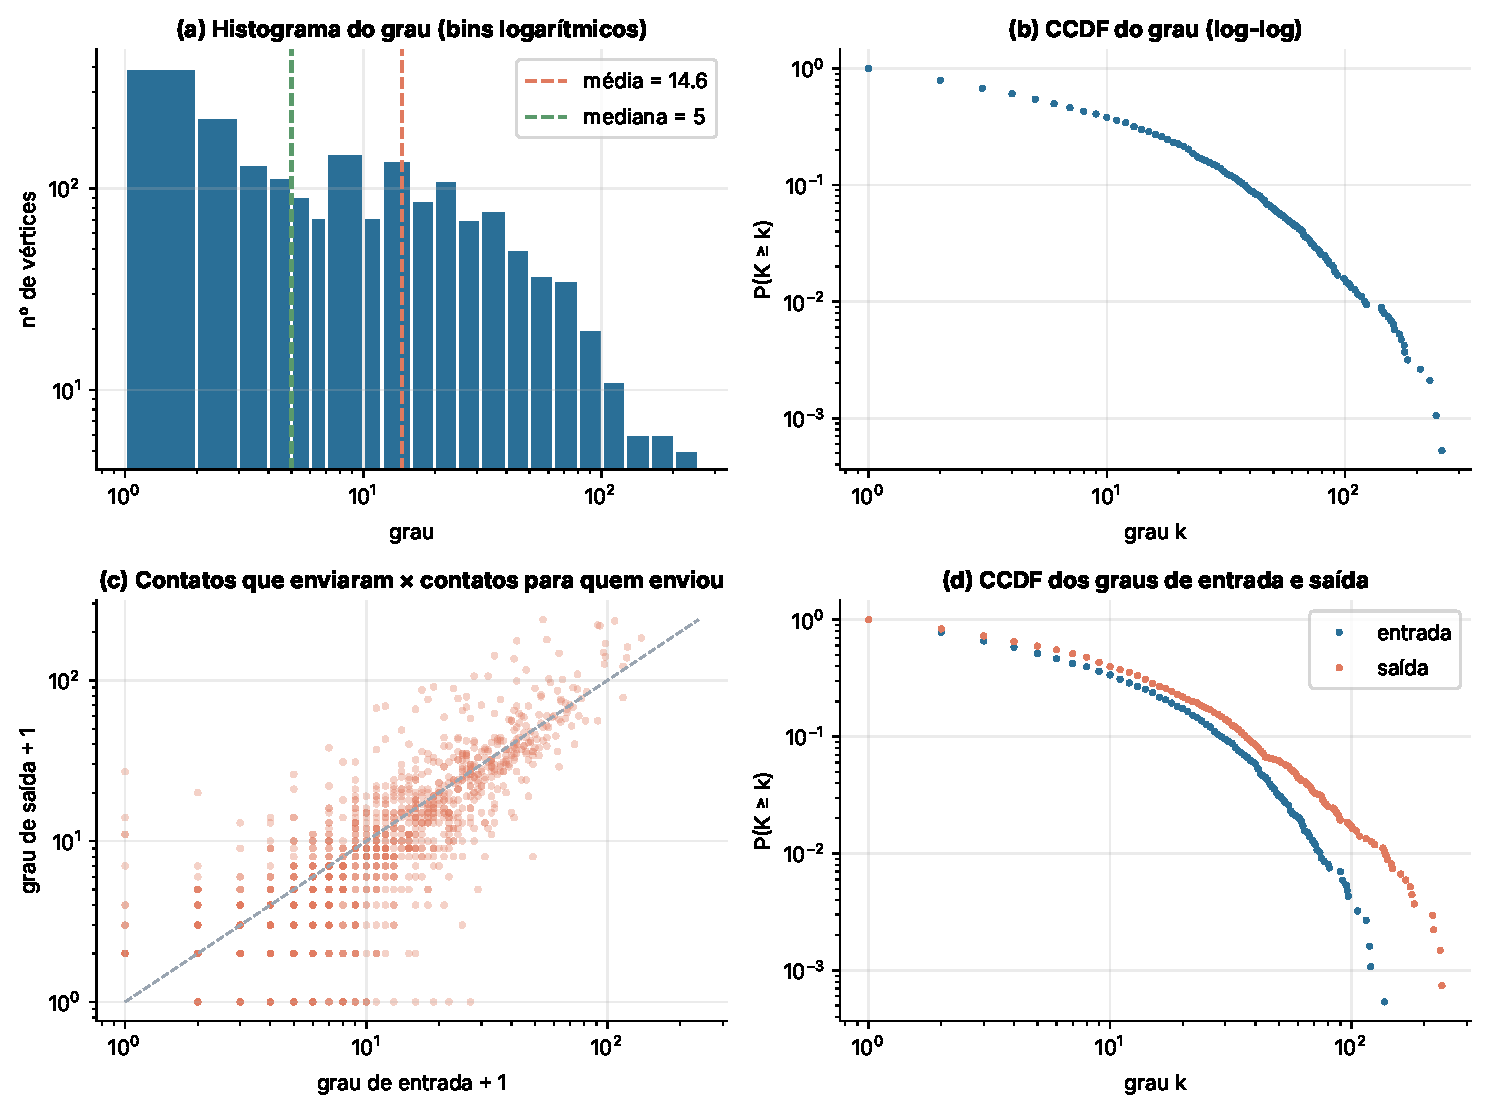
\includegraphics[width=\columnwidth]{figuras/distribuicao_graus.pdf}
  \caption{Distribuição de graus (não dirigido). A maioria dos usuários tem poucos contatos e uns poucos chegam a mais de 250.}
  \Description{Histograma e distribuição acumulada complementar dos graus em escala logarítmica.}
  \label{fig:graus}
\end{figure}

A maior componente tem diâmetro \diametro, raio \raio{} e caminho médio \caminhoMedio{} (Figura~\ref{fig:dist}): quase qualquer par de usuários está a três ou quatro passos. A clusterização média é \clustMedio{} e a transitividade, \transitividade{}; a diferença indica que os vértices de grau baixo, que dominam a média local, fecham triângulos com mais frequência que os hubs. A assortatividade negativa (\assortatividade{}) mostra que hubs se conectam a vértices de grau baixo, o que combina com um padrão de envio em massa (Tabela~\ref{sec:desc}). O núcleo $k$ máximo é \coreMax{} (Figura~\ref{fig:kcore}). A reciprocidade de \reciprocidade{} indica que a maioria dos pares que se escrevem recebe resposta.

\begin{figure}[t]
  \centering
  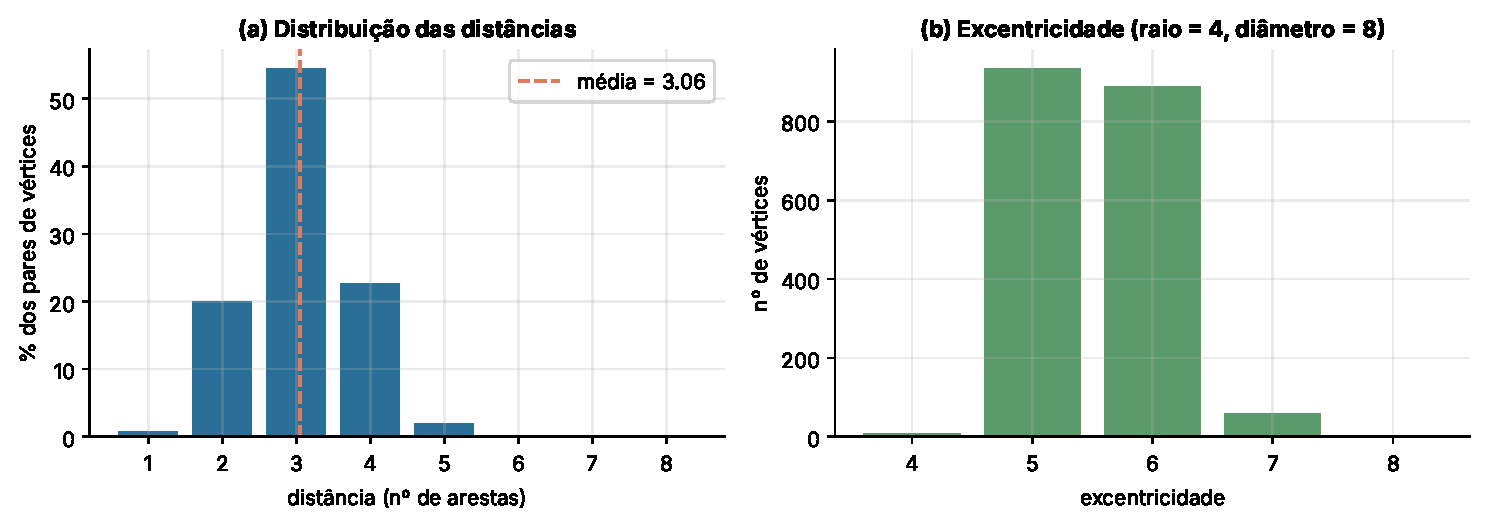
\includegraphics[width=\columnwidth]{figuras/distancias.pdf}
  \caption{Distribuição das distâncias entre pares na maior componente.}
  \Description{Histograma das distâncias, com pico em três passos.}
  \label{fig:dist}
\end{figure}

\begin{figure}[t]
  \centering
  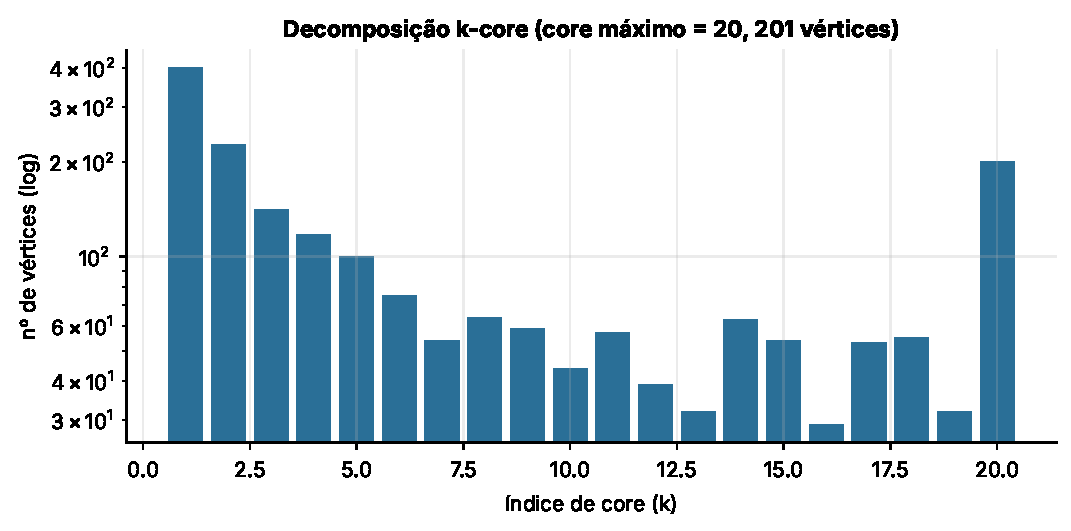
\includegraphics[width=\columnwidth]{figuras/kcore.pdf}
  \caption{Tamanho dos núcleos $k$. O núcleo mais denso tem 201 vértices e $k=\coreMax$.}
  \Description{Gráfico do número de vértices por valor de k-core.}
  \label{fig:kcore}
\end{figure}

\begin{figure}[t]
  \centering
  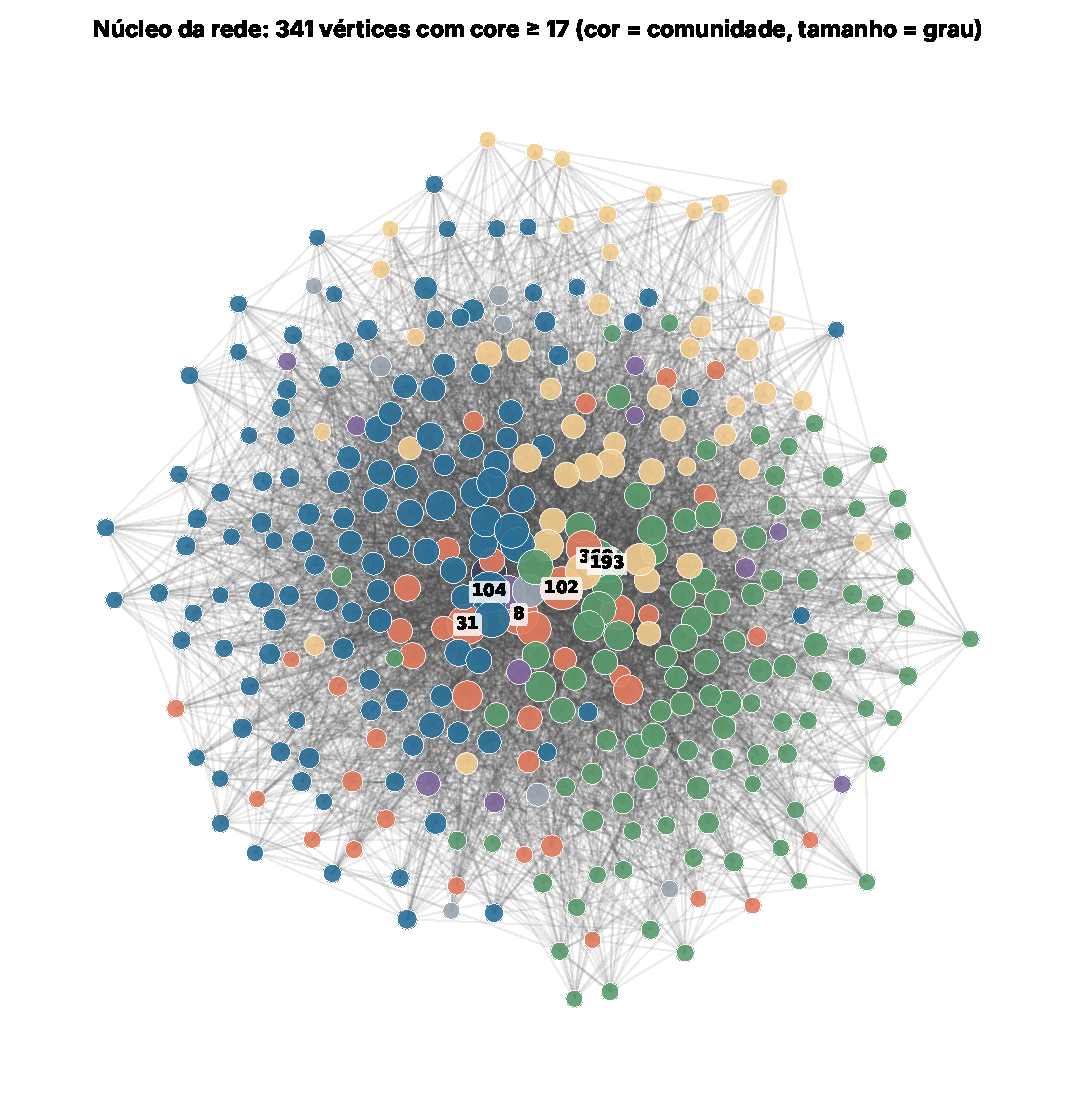
\includegraphics[width=\columnwidth]{figuras/grafo_nucleo.pdf}
  \caption{Visualização do núcleo da rede (vértices com $k$-core $\ge17$). O grafo completo é ilegível; esta versão reduzida mostra a região densa.}
  \Description{Desenho do subgrafo do núcleo, com vértices maiores para graus maiores.}
  \label{fig:nucleo}
\end{figure}

Figura~\ref{fig:nucleo} mostra o núcleo da rede. Todas as medidas obrigatórias foram calculadas; nenhuma precisou ser aproximada.

%--------------------------------------------------------------------
\section{Resultados: Parte II}
Tabela~\ref{tab:tempos} reúne a complexidade teórica e os tempos medidos. Os resultados foram validados entre si: Dijkstra, Bellman--Ford e Floyd--Warshall retornam as mesmas distâncias, e Prim e Kruskal, a mesma árvore geradora mínima, de peso \pesoMST{}.

\paragraph{Resultados dos algoritmos.} BFS e DFS alcançam os \tamMaiorComp{} vértices da maior componente. O grafo \emph{não} é euleriano: há \grausImpares{} vértices de grau ímpar na maior componente (e 1.692 vértices com grau de entrada diferente do de saída no grafo dirigido). Bellman--Ford não encontra ciclo negativo (os pesos são positivos) e converge em poucas passadas (7 a 8), muito abaixo do pior caso de $V-1$, graças à parada antecipada. O algoritmo de Tarjan encontra \nSCC{} componentes fortemente conexas, sendo a maior com \maiorSCC{} vértices e 595 isoladas, além de \nPontes{} pontes e \nArticulacoes{} pontos de articulação, que são fragilidades estruturais relevantes para a Parte III.

\begin{table*}
  \caption{Tempo de execução (média, desvio-padrão e IC de 95\%) na maior componente ($n=1893$, $m=13835$) e complexidade teórica. IC pela Normal quando $n\ge30$ e pela t-Student quando $n<30$.}
  \label{tab:tempos}
  \small
  \begin{tabular}{llrrrl}
    \toprule
    Algoritmo & Complexidade & Rep. & Média & DP & IC 95\% \\
    \midrule
    BFS & $O(V + E)$ & 30 & 1,09 ms & 0,17 ms & [1,03 ms; 1,15 ms] \\
    DFS & $O(V + E)$ & 30 & 1,77 ms & 0,38 ms & [1,64 ms; 1,91 ms] \\
    Eulerianidade & $O(V + E)$ & 30 & 1,37 ms & 0,22 ms & [1,29 ms; 1,45 ms] \\
    Dijkstra & $O((V + E) \log V)$ & 30 & 4,32 ms & 0,54 ms & [4,13 ms; 4,51 ms] \\
    Bellman-Ford & $O(V\cdot E)$ & 30 & 14,00 ms & 1,22 ms & [13,56 ms; 14,43 ms] \\
    Tarjan (SCC) & $O(V + E)$ & 30 & 2,82 ms & 0,27 ms & [2,73 ms; 2,92 ms] \\
    Tarjan (pontes) & $O(V + E)$ & 30 & 3,80 ms & 0,39 ms & [3,66 ms; 3,94 ms] \\
    Kruskal & $O(E \log E)$ & 30 & 7,88 ms & 0,79 ms & [7,60 ms; 8,16 ms] \\
    Prim & $O(E \log V)$ & 30 & 13,27 ms & 0,95 ms & [12,94 ms; 13,61 ms] \\
    Floyd-Warshall & $O(V^3)$ & 5 & 23,62 s & 1,25 s & [22,07 s; 25,18 s] \\
    Floyd-Warshall ($n=150$, python) & $O(V^3)$ & 10 & 206,25 ms & 34,04 ms & [181,91 ms; 230,60 ms] \\
    Floyd-Warshall ($n=150$, numpy) & $O(V^3)$ & 10 & 4,48 ms & 0,17 ms & [4,36 ms; 4,61 ms] \\
    \bottomrule
  \end{tabular}
\end{table*}


\paragraph{Tempos.} Os algoritmos lineares são os mais rápidos (BFS $\approx$1,1\,ms); Dijkstra, Kruskal e Prim ficam entre 4 e 13\,ms, e Bellman--Ford, em 14\,ms, é o mais lento dos algoritmos de fonte única. Floyd--Warshall é cúbico: no grafo inteiro, com a versão vetorizada, leva cerca de 24\,s (a matriz de 1893$^2$ distâncias ocupa $\approx$29\,MB com 64 bits). Em $n=150$, a versão em Python puro (206\,ms) é cerca de 46 vezes mais lenta que a vetorizada (4,5\,ms) com a mesma complexidade, o que mostra que a constante importa. Os tempos dependem do computador usado (Figura~\ref{fig:tempos}).

\begin{table}
  \caption{Inclinação do ajuste log-log do tempo observado em função da expressão teórica (por exemplo, $V+E$). Valor 1 indica que o tempo cresce como a fórmula prevê.}
  \label{tab:inclinacoes}
  \small
  \begin{tabular}{llr}
    \toprule
    Algoritmo & Teórica & Inclinação \\
    \midrule
    BFS & $V + E$ & 0,94 \\
    DFS & $V + E$ & 0,87 \\
    Dijkstra & $(V+E) \log V$ & 0,81 \\
    Bellman-Ford & $V\cdot E$ & 0,65 \\
    Kruskal & $E \log E$ & 0,89 \\
    Prim & $E \log V$ & 1,00 \\
    Tarjan (pontes) & $V + E$ & 1,01 \\
    Floyd-Warshall & $V^3$ & 0,99 \\
    \bottomrule
  \end{tabular}
\end{table}


\paragraph{Complexidade observada.} Para cada algoritmo, ajustamos uma reta a $\log(\text{tempo})$ em função do logaritmo da expressão teórica (por exemplo, $V+E$ para a BFS), em amostras de vértices de tamanho crescente (de 100 até $n$). Uma inclinação próxima de 1 indica que o tempo cresce como a fórmula prevê. Tabela~\ref{tab:inclinacoes} e Figura~\ref{fig:complex} mostram inclinações entre 0,87 e 1,01 para BFS, DFS, Kruskal, Prim, Tarjan e Floyd--Warshall (para este, o tempo vai de 2,7\,ms com 100 vértices a 1,25\,s com 800, crescimento cúbico). Dijkstra (0,81) e, principalmente, Bellman--Ford (0,65) ficam abaixo de 1: no caso do Bellman--Ford, a parada antecipada faz o algoritmo terminar em poucas passadas, e não nas $V-1$ do pior caso; o valor $V\cdot E$ da teoria é, portanto, um limite superior pessimista para este grafo. As amostras de vértices alteram também a razão $m/n$, o que pode afetar os ajustes dos algoritmos lineares.% REVISAR: interpretação a confirmar/reescrever com as próprias palavras

\begin{figure}[t]
  \centering
  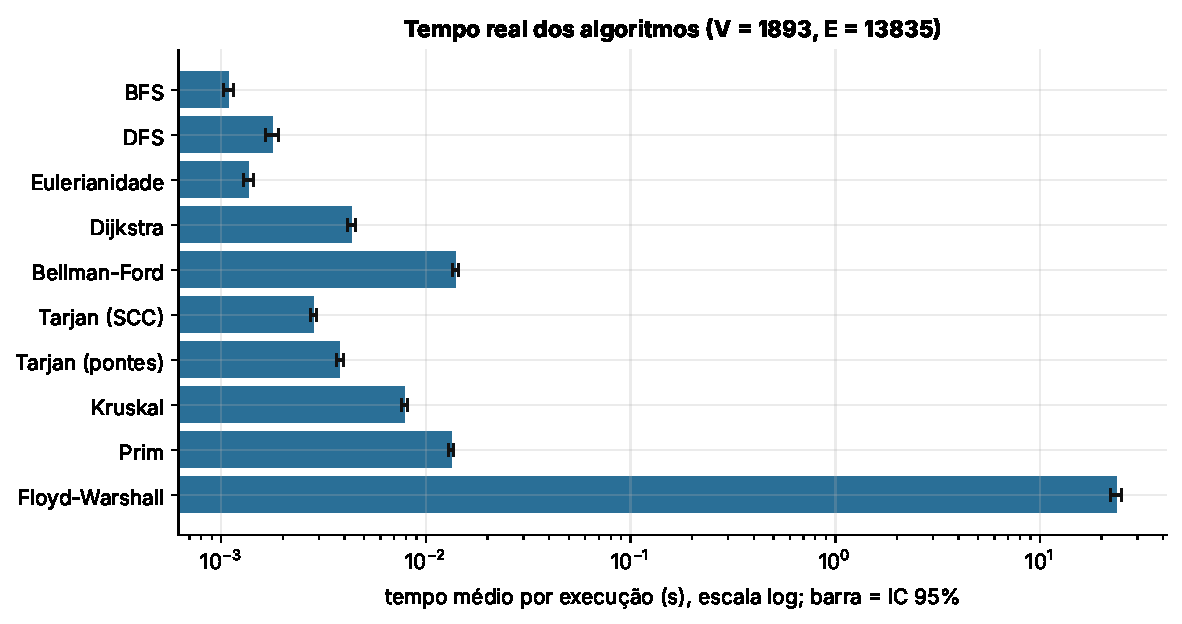
\includegraphics[width=\columnwidth]{figuras/tempos_algoritmos.pdf}
  \caption{Tempo médio de cada algoritmo na maior componente (com IC de 95\%).}
  \Description{Gráfico de barras com os tempos médios por algoritmo, em escala logarítmica.}
  \label{fig:tempos}
\end{figure}

\begin{figure*}[t]
  \centering
  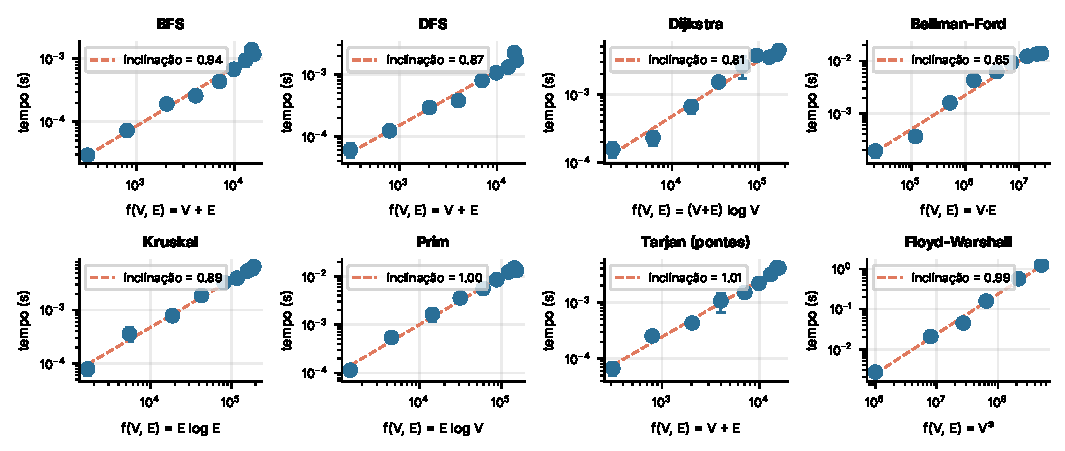
\includegraphics[width=\textwidth]{figuras/complexidade_observada.pdf}
  \caption{Tempo observado versus tamanho da amostra (escala log-log), com a curva teórica ajustada.}
  \Description{Painéis com o tempo em função do tamanho para cada algoritmo, em escala log-log.}
  \label{fig:complex}
\end{figure*}

%--------------------------------------------------------------------
\section{Resultados: Parte III}

\subsection{Questão 1: a rede é um mundo pequeno?}
\textbf{Sim em relação ao grafo aleatório; só parcialmente em relação ao nulo de mesmos graus.} A maior componente tem $C=0{,}1097$ e $L=\caminhoMedio$. Contra $G(n,m)$, $C/C_{al}=\razaoCER$ e $L/L_{al}=\razaoLER$, portanto $L\approx L_{al}$ e $C\gg C_{al}$, com $\sigma\approx\sigmaER$ (Tabela~\ref{tab:smallworld}, Figura~\ref{fig:sw}). Pelo critério do enunciado, a rede é um mundo pequeno.

\begin{table}
  \caption{Teste de mundo pequeno na maior componente. Médias de 20 amostras de cada modelo nulo (distâncias estimadas com 500 fontes).}
  \label{tab:smallworld}
  \small
  \begin{tabular}{lrrrr}
    \toprule
    Grafo & $C$ & $L$ & $C/C_{al}$ & $L/L_{al}$ \\
    \midrule
    Observado & 0,1097 & 3,055 & -- & -- \\
    Aleatório $G(n,m)$ & 0,0076 & 3,083 & 14,4 & 0,991 \\
    Mesmos graus & 0,0885 & 3,037 & 1,24 & 1,006 \\
    \bottomrule
  \end{tabular}
\end{table}


Esse resultado é, porém, inflado pela presença de hubs, pois $G(n,m)$ não reproduz a heterogeneidade de graus. Contra o nulo que preserva a sequência de graus, $C/C_{al}=\razaoCGrau$ e $L/L_{al}=\razaoLGrau$, e $\sigma$ cai para \sigmaGrau{}. A maior parte do agrupamento, portanto, \emph{decorre da distribuição de graus}, e só uma parcela pequena (cerca de 24\%) é estrutura adicional. Na prática, a rede é de fato bem conectada por poucos passos, mas o agrupamento não indica comunidades fortes por si só.% REVISAR: interpretação

\begin{figure}[t]
  \centering
  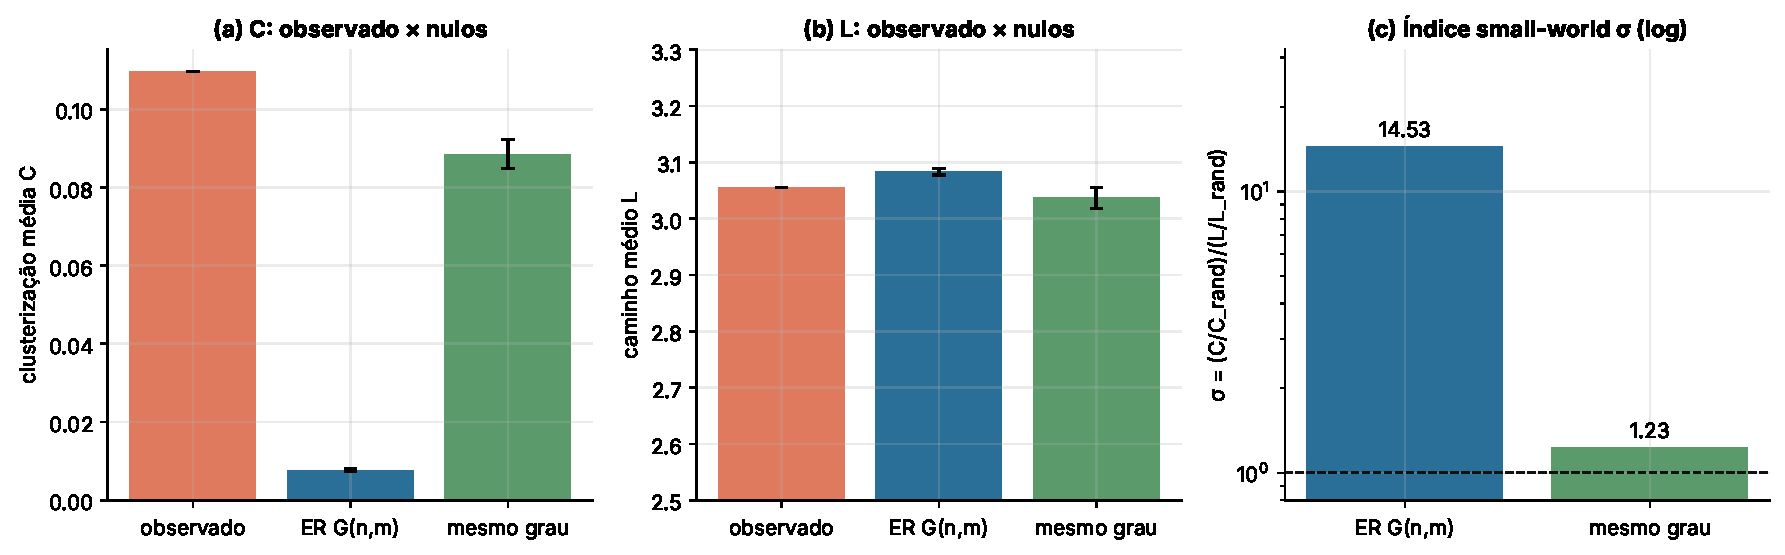
\includegraphics[width=\columnwidth]{figuras/smallworld.pdf}
  \caption{Comparação de $C$, $L$ e $\sigma$ com os dois modelos nulos.}
  \Description{Barras com os valores de C, L e sigma para a rede observada e os nulos.}
  \label{fig:sw}
\end{figure}

\subsection{Questão 2: a distribuição de graus segue uma lei de potência?}
\textbf{Não.} Uma regressão linear em escala log-log sobre $P(k)$ daria $\gamma\approx\gammaOLS$, valor abaixo de 2 e que não corresponde a uma distribuição normalizável; essa regressão é enviesada pela cauda ruidosa e \emph{não} deve ser usada. A estimativa por máxima verossimilhança, com $k_{\min}=\kminPL$ escolhido por KS e \nCaudaPL{} vértices na cauda, dá $\gamma=\gammaPL$, mas o teste de \emph{bootstrap} rejeita a hipótese ($p=\pvalorPL<0{,}1$). A razão de verossimilhanças favorece a lognormal ($R=\RLognormal$, $p=\pLognormal$) e não distingue a exponencial ($R=\RExponencial$, $p=\pExponencial$) (Figura~\ref{fig:pl}). Além disso, $\gamma$ não é estável: ao variar $k_{\min}$ de 1 a 30, vai de 1,44 a 2,72. Conclusão: a cauda é pesada, mas a lei de potência não é um bom modelo. Implicação: previsões baseadas em redes livres de escala (por exemplo, ausência de limiar de percolação) não se aplicam diretamente.

\begin{figure*}[t]
  \centering
  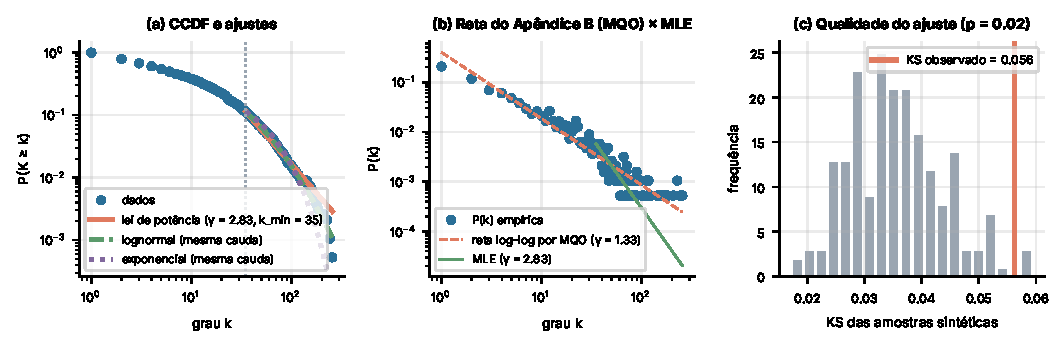
\includegraphics[width=\textwidth]{figuras/lei_de_potencia.pdf}
  \caption{Distribuição de graus em escala log-log com os ajustes: máxima verossimilhança na cauda e regressão por mínimos quadrados.}
  \Description{CCDF dos graus com os ajustes de lei de potência, lognormal e exponencial.}
  \label{fig:pl}
\end{figure*}

\subsection{Questão 3: robustez a falhas e ataques}
\textbf{A rede é robusta a falhas aleatórias e frágil a ataques a hubs.} Removendo $r=\nRemovidos$ vértices ao acaso (30 repetições), a maior componente mantém \AAleatorio{} dos vértices ($A_{rel}=\ARelAleatorio$ da componente original), e o caminho médio quase não muda (\CAleatorio{}). Com o mesmo número de remoções dirigidas, A cai para \AAtaqueGrau{} (grau), \AAtaqueInterm{} (intermediação) e \AAtaquePR{} (PageRank), o número de componentes sobe para 228--339 (contra cerca de 21 na remoção aleatória), o caminho médio sobe para até \CAtaqueGrau{} e até \DAtaqueInterm{} dos vértices ficam isolados (Tabela~\ref{tab:robustez}, Figuras~\ref{fig:rob} e~\ref{fig:curvas}).

\begin{table*}
  \caption{Robustez após remover $r=95$ vértices (5\% de $n$). A: fração na maior componente; B: nº de componentes; C: caminho médio na maior componente; D: fração de vértices isolados.}
  \label{tab:robustez}
  \small
  \begin{tabular}{lrrrr}
    \toprule
    Remoção & A & B & C & D \\
    \midrule
    Íntegro & 1,000 & 1 & 3,055 & 0,0\% \\
    Aleatória ($\pm$ DP) & 0,939 $\pm$ 0,005 & 20,8 $\pm$ 8,5 & 3,064 $\pm$ 0,015 & 1,1\% \\
    Ataque: grau & 0,793 & 289 & 3,795 & 15,6\% \\
    Ataque: intermediação & 0,763 & 339 & 3,698 & 18,1\% \\
    Ataque: PageRank & 0,827 & 228 & 3,618 & 12,3\% \\
    \bottomrule
  \end{tabular}
\end{table*}


A intermediação é a estratégia mais danosa para A, B e D; o PageRank é a menos danosa dentre as três. Nas curvas até 30\% de remoção, a maior componente com remoção aleatória ainda tem 65\% dos vértices, mas, com remoção por grau, cai para 4\% (e por intermediação, para 10\%). O padrão é típico de redes heterogêneas~\cite{albert2000}. Implicação: se os hubs forem o alvo (contas desativadas, por exemplo), a rede se fragmenta com rapidez; a proteção deve se concentrar neles.

\begin{figure*}[t]
  \centering
  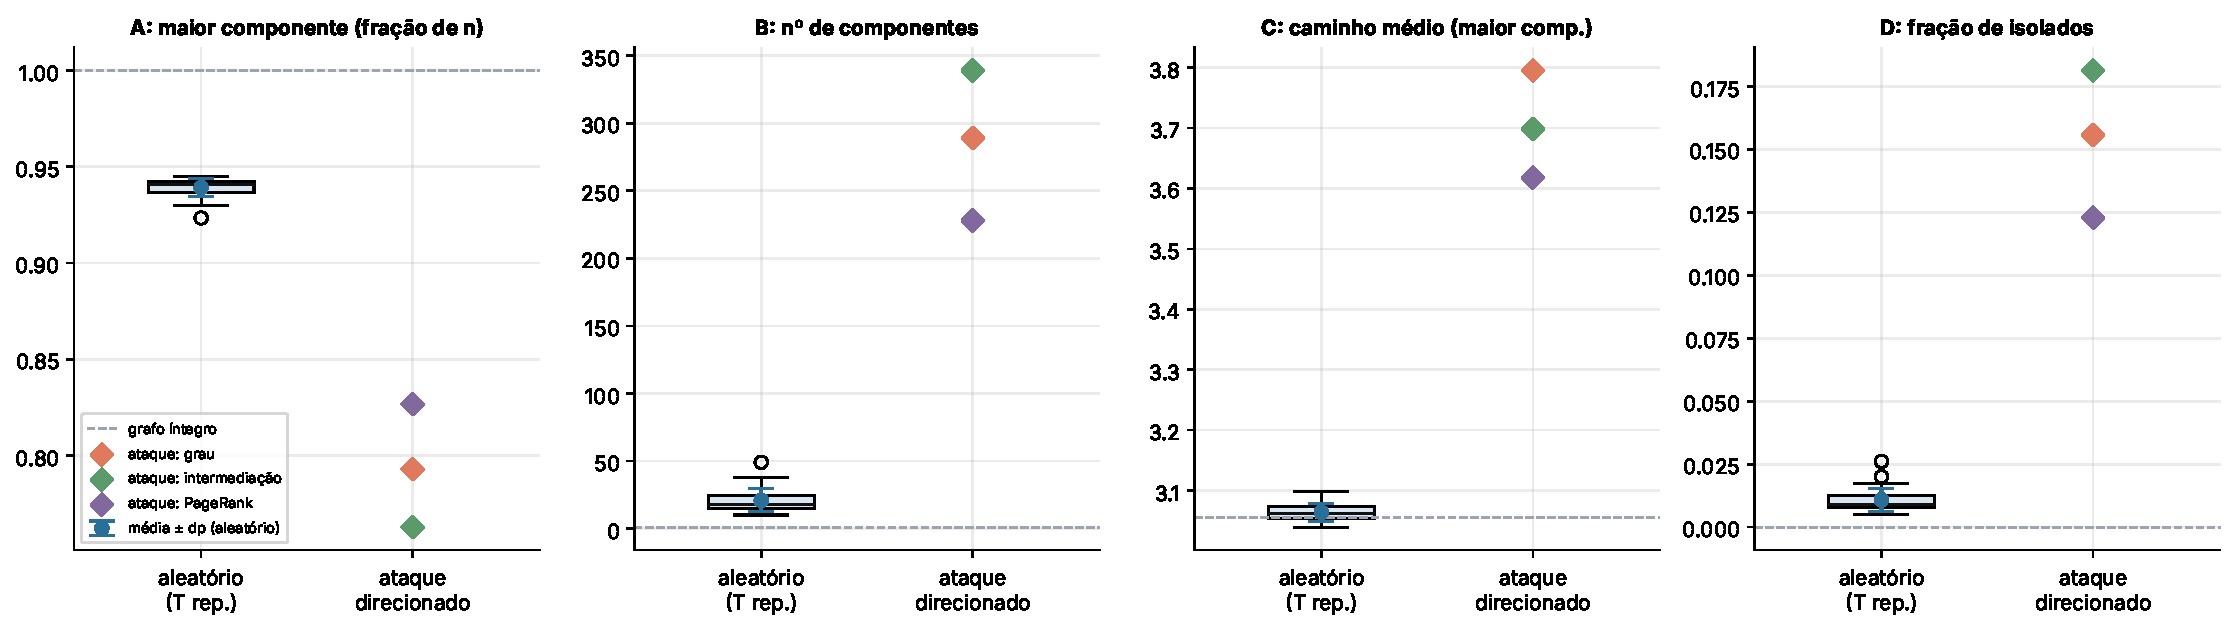
\includegraphics[width=\textwidth]{figuras/robustez_boxplot.pdf}
  \caption{Métricas A--D após remover 5\% dos vértices. \emph{Boxplots}: 30 remoções aleatórias; marcadores: ataques com ranking fixo.}
  \Description{Boxplots das quatro métricas de robustez para remoção aleatória e pontos para os ataques.}
  \label{fig:rob}
\end{figure*}

\begin{figure}[t]
  \centering
  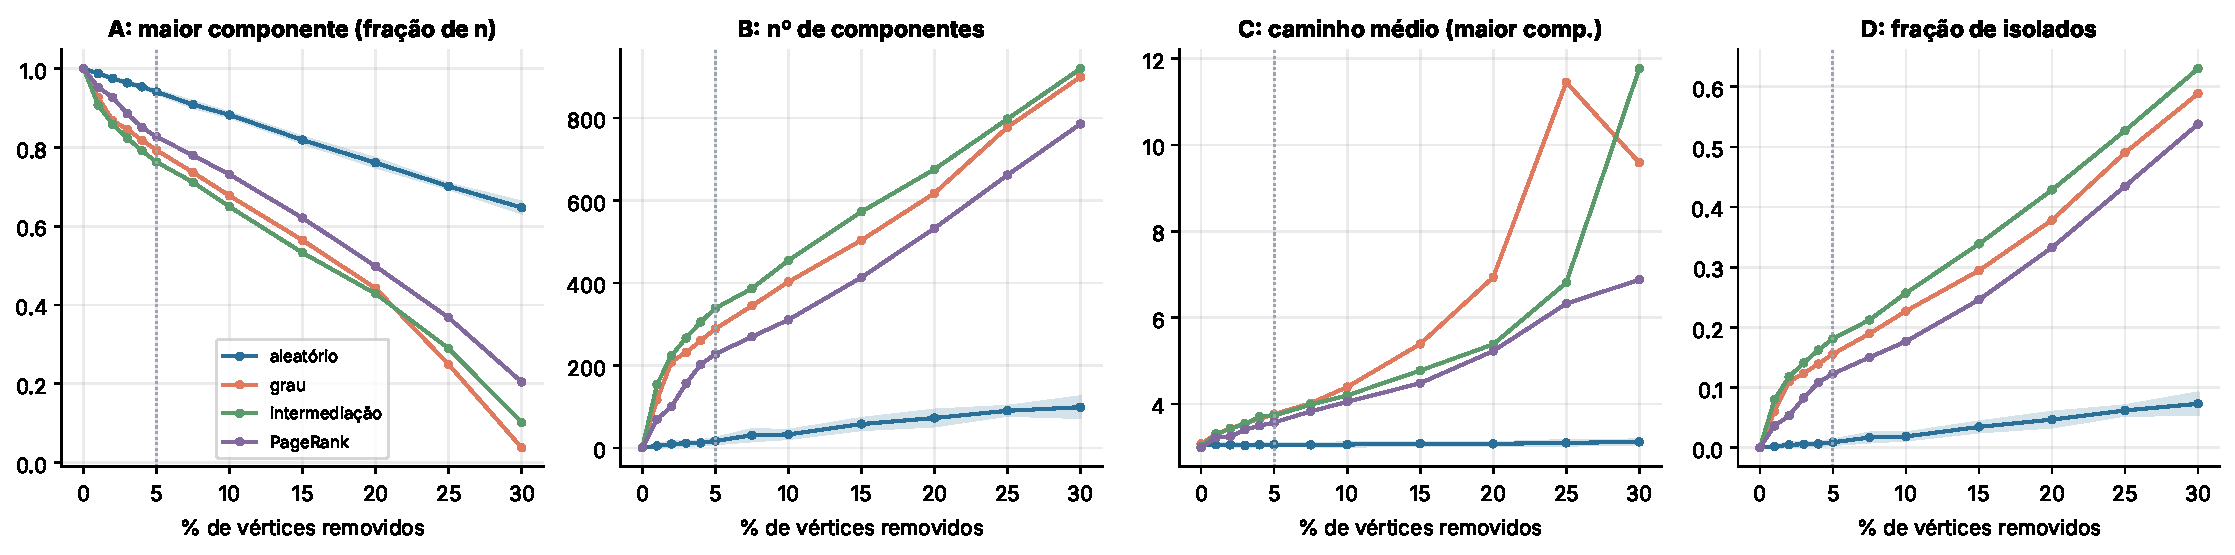
\includegraphics[width=\columnwidth]{figuras/robustez_curvas.pdf}
  \caption{Fração na maior componente conforme a fração removida (até 30\%).}
  \Description{Curvas de fragmentação para remoção aleatória e para os três ataques.}
  \label{fig:curvas}
\end{figure}

\subsection{Questão 4: descoberta mais interessante}
\label{sec:desc}
\textbf{Os hubs da rede são remetentes em massa, não participantes de conversas.} Entre os 20 usuários de maior grau, o grau de saída médio é cerca de 159 contra 80 de entrada, e apenas 43\% de seus destinatários respondem, contra 64\% no conjunto da rede. A reciprocidade cai com o grau, de 74--79\% para graus entre 2 e 31, até 44\% para grau $\ge128$ (Figura~\ref{fig:desc}). Os 5\% de usuários que mais enviam produzem \topCincoMsgs{} das mensagens. Isso explica a assortatividade negativa e a fragilidade a ataques: os hubs sustentam a conectividade, mas não por laços recíprocos. A rede de mensagens privadas é, em suma, mais um sistema de difusão a partir de poucos emissores do que um conjunto de conversas simétricas. Outros números: 38\% dos pares trocam uma única mensagem, e os pares com 10 ou mais mensagens (cerca de 10\% dos pares) concentram 46\% do tráfego; a mediana entre a primeira mensagem de cada sentido em pares recíprocos (6.458) é de 3,9\,h.% REVISAR: interpretação do padrão de envio em massa

\begin{figure*}[t]
  \centering
  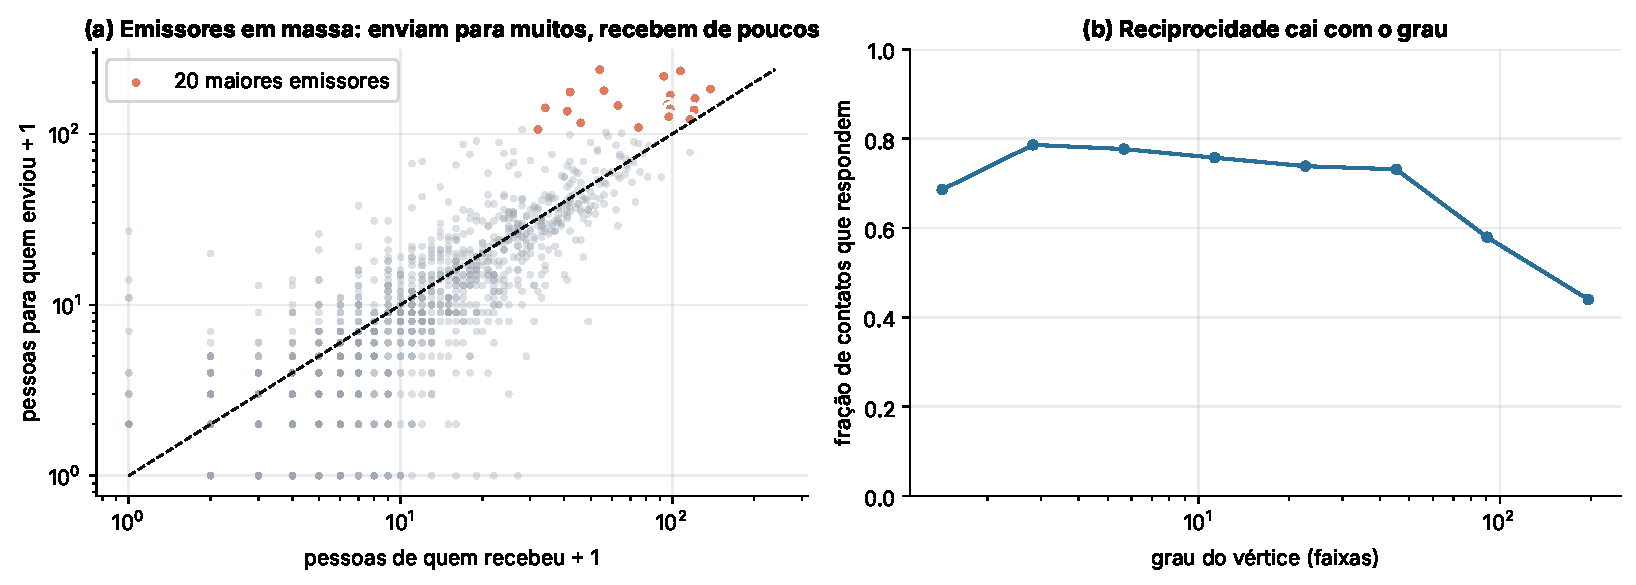
\includegraphics[width=\textwidth]{figuras/descobertas.pdf}
  \caption{Comportamento dos hubs: reciprocidade por faixa de grau e concentração das mensagens.}
  \Description{Painéis com reciprocidade por faixa de grau, concentração do envio e contatos de um hub.}
  \label{fig:desc}
\end{figure*}

\subsection{Questão extra: modelos clássicos}
Comparamos a rede com os modelos de Erd\H{o}s--R\'enyi, Barab\'asi--Albert~\cite{barabasi1999} e Watts--Strogatz~\cite{watts1998}, com o mesmo número de vértices e arestas aproximado (Tabela~\ref{tab:modelos}, Figura~\ref{fig:mod}). Nenhum se ajusta bem. O ER subestima o agrupamento e os hubs ($C=0{,}008$, $k_{\max}\approx29$); o BA produz hubs (cerca de 197) mas agrupamento baixo ($C\approx0{,}031$); o WS exagera o agrupamento ($C=0{,}51$) e tem caminhos mais longos ($L=4{,}14$). O nulo de mesmos graus é o mais próximo ($C=0{,}089$, $L=3{,}03$), o que reforça que a heterogeneidade de graus explica a maior parte da estrutura.

\begin{table}
  \caption{Grafo observado e modelos clássicos de mesma ordem e tamanho aproximado (médias de réplicas). KS: distância de Kolmogorov--Smirnov entre as distribuições de grau.}
  \label{tab:modelos}
  \small
  \begin{tabular}{lrrrrr}
    \toprule
    Modelo & $C$ & $L$ & $k_{\max}$ & DP grau & KS \\
    \midrule
    Observado & 0,110 & 3,06 & 255 & 24,5 & 0,00 \\
    Erd\H{o}s--R\'enyi & 0,008 & 3,08 & 29 & 3,8 & 0,55 \\
    Barab\'asi--Albert & 0,031 & 2,91 & 197 & 14,5 & 0,54 \\
    Watts--Strogatz & 0,509 & 4,14 & 19 & 1,2 & 0,64 \\
    Mesmos graus & 0,089 & 3,03 & 255 & 24,5 & 0,00 \\
    \bottomrule
  \end{tabular}
\end{table}


\begin{figure*}[t]
  \centering
  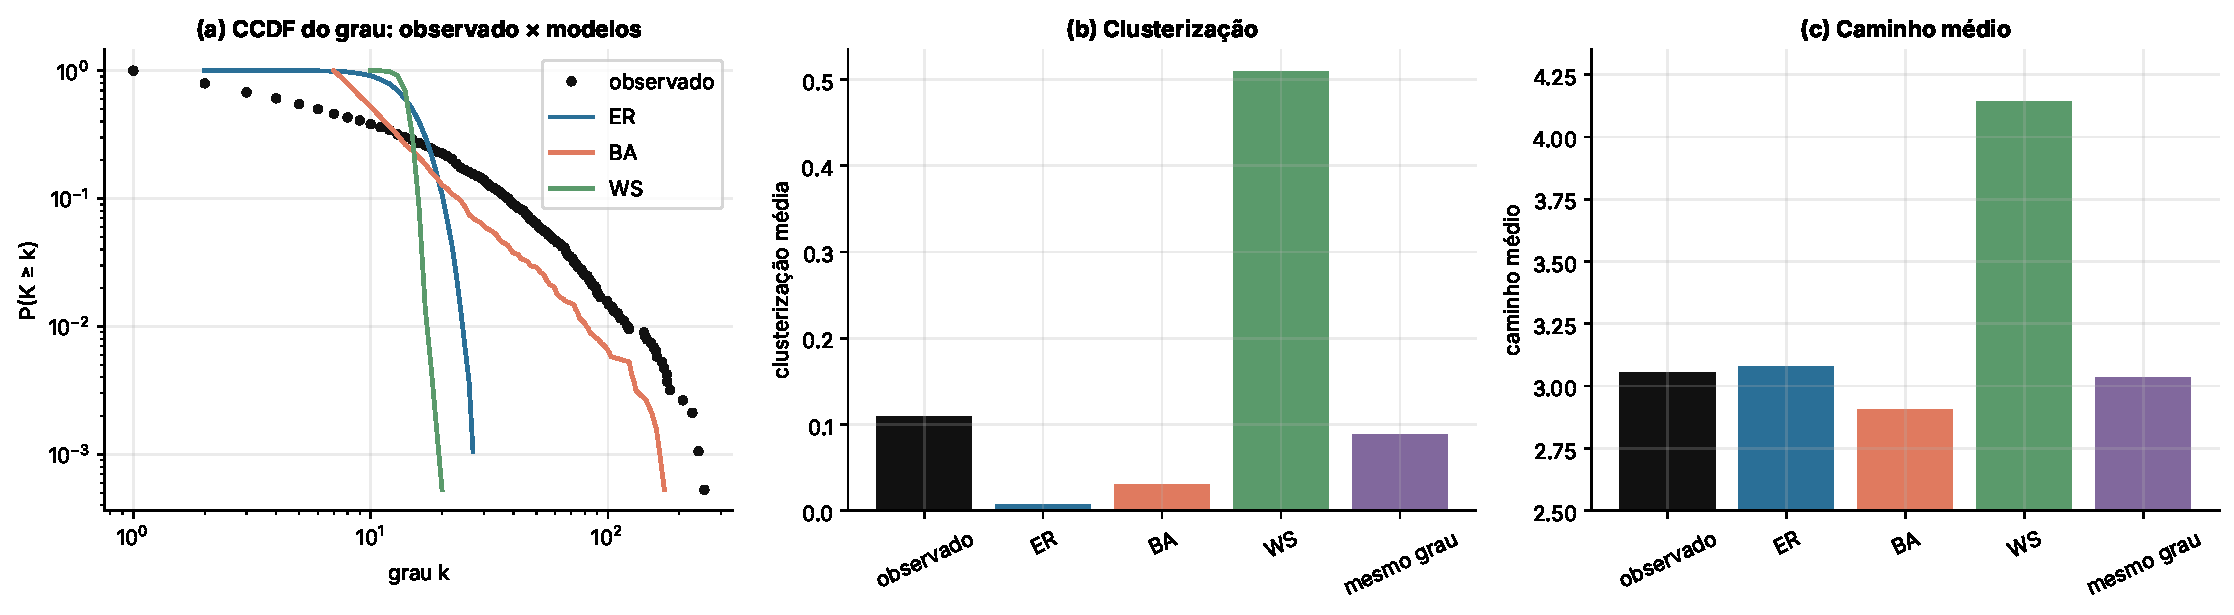
\includegraphics[width=\textwidth]{figuras/modelos_classicos.pdf}
  \caption{Rede observada e modelos clássicos: distribuição de graus, $C$ e $L$.}
  \Description{Comparação visual entre a rede e os modelos ER, BA e WS.}
  \label{fig:mod}
\end{figure*}

%--------------------------------------------------------------------
\section{Discussão crítica}
\paragraph{Limitações.} (i) Ao colapsar o grafo temporal em um grafo estático, perdemos a ordem das mensagens; caminhos que passam por arestas ``fora de ordem no tempo'' podem não ser realizáveis. (ii) O peso $w=1/m$ é uma escolha de modelagem, e outras funções dariam outras distâncias ponderadas, ainda que não alterem as medidas não ponderadas. (iii) As razões de mundo pequeno dependem do nulo; reportamos dois. (iv) Os tempos da Parte II dependem do computador e do interpretador, e as inclinações log-log sofrem do efeito de amostras de vértices cuja densidade varia. (v) A rede cobre um comportamento específico de uma rede social de estudantes.

\paragraph{Reprodutibilidade.} O pipeline completo roda por \texttt{scripts/run\_all.py}, com semente fixa; os números do texto vêm de \texttt{macros.tex} e das tabelas geradas, e não foram digitados à mão.

\section{Conclusão}
O grafo CollegeMsg é esparso, assortativo negativo e de caminhos curtos. Seu agrupamento é alto em relação ao acaso, mas em grande parte consequência da distribuição de graus; a lei de potência é rejeitada, e a lognormal ajusta melhor a cauda. A rede resiste a falhas aleatórias, mas se fragmenta rapidamente sob ataques a hubs, que são remetentes em massa com baixa reciprocidade. Os algoritmos implementados concordam com o NetworkX, e os tempos medidos são compatíveis com as complexidades teóricas, com ressalvas sobre o ajuste log-log. Como trabalho futuro, uma análise que respeite a ordem temporal (caminhos temporais) e a busca de comunidades.

%\begin{acks}
%\end{acks}

\bibliographystyle{ACM-Reference-Format}
\bibliography{refs}

\end{document}
